\documentclass[
%% TIKZ_CLASSOPTION %%
tikz
]{standalone}
\usepackage{amsmath}
\usetikzlibrary{matrix}
%% EXTRA_TIKZ_PREAMBLE_CODE %%
\usepackage{amsmath}
\usepackage{amssymb}
\usepackage{xcolor}
\usetikzlibrary{positioning, calc}
\begin{document}
%% TIKZ_CODE %%
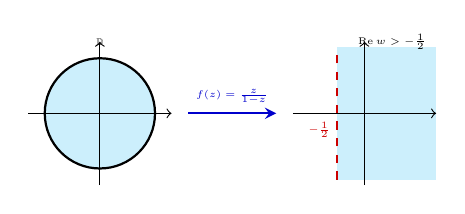
\begin{tikzpicture}[scale=0.7, every node/.style={transform shape}, region/.style={fill=cyan!20}, arrow/.style={->, >=stealth, thick, blue!80!black}]
  \begin{scope}[shift={(0,0)}]
    \fill[region] (0,0) circle (1);
    \draw[->, black] (-1.3,0) -- (1.3,0); 
    \draw[->, black] (0,-1.3) -- (0,1.3);
    \draw[thick, black] (0,0) circle (1);
    \node at (0, 1.3) [font=\tiny\bfseries] {$\mathbb{D}$};
  \end{scope}
  
  \draw[arrow] (1.6,0) -- node[above=1pt] {\tiny $f(z)=\frac{z}{1-z}$} (3.2,0);
  
  \begin{scope}[shift={(4.8,0)}]
    \fill[region] (-0.5,-1.2) rectangle (1.3,1.2);
    \draw[->, black] (-1.3,0) -- (1.3,0); 
    \draw[->, black] (0,-1.3) -- (0,1.3);
    \draw[dashed, thick, red!80!black] (-0.5,-1.2) -- (-0.5,1.2);
    \node at (-0.5,-0.3) [font=\tiny, left, red!80!black] {$-\frac{1}{2}$};
    \node at (0.5, 1.3) [font=\tiny\bfseries] {$\operatorname{Re} w > -\frac{1}{2}$};
  \end{scope}
\end{tikzpicture}
\end{document}
